%****************************************************************************%
%* DIET User's Manual JXTA chapter file                                     *%
%*                                                                          *%
%*  Author(s):                                                              *%
%*    - Cedric TEDESCHI (Cedric.Tedeschi@insa-lyon.fr)                      *%
%*                                                                          *%
%* $LICENSE$                                                                *%
%****************************************************************************%
%* $Id$
%* $Log$
%* Revision 1.12  2008/04/07 22:25:38  ecaron
%* Updated files to pdflatex compilation
%*
%* Revision 1.11  2006/12/04 12:18:35  dloureir
%* minor corrections
%*
%* Revision 1.10  2006/12/04 10:10:36  ctedesch
%* correct typos and update for cmake
%*
%* Revision 1.9  2006/12/04 09:49:32  ctedesch
%* add old logs in header
%*
%* Revision 1.8  2006/12/04 09:42:57  ctedesch
%* header
%*
%* Revision 1.7  2005/06/01 07:21:35  alsu
%* fixing a figure labeling problem
%* 
%* Revision 1.6 2004/08/27 17:04:36  ctedesch
%* - update DIET J chapter :
%* use of the PIF DIET
%* JXTA -> DIET J
%*
%* - syntax corrections in data chapter (_ -> \_)
%* 
%* Revision 1.5  2004/07/09 19:51:58  ctedesch
%* - javac and javah detected instead of java
%* - JXTA_LIB automatically set before compilation
%* - JXTA libraries copied into install_dir/lib
%* - DIET license added in the java files
%* - JXTA loaders scripts modified: set JXTA_LIB for execution
%* - update doc
%* Revision 1.4 2004/07/06 13:40:42  ctedesch
%* add corrections from Raphael Bolze.
%*
%* Revision 1.3 2004/06/16 19:08:19  ctedesch
%* corrections about JXTA release to use
%*
%* Revision 1.2 2004/06/16 12:58:19  ctedesch
%* change information concerning JXTA release to use
%*
%* Revision 1.1  2004/06/16 09:06:03  ctedesch
%* add chapter called P2P DIET extension to the DIET user's manual
%****************************************************************************%

\chapter{P2P DIET extension: DIET$_{J}$}
\label{ch:p2pextension}

To extend the field of the available services for each client in a
transparent manner, DIET uses the Multi-Agent system to increase
scalability. To achieve this, the MAs access each others' resources
when processing a client's request. Thus, each request is not only
submitted inside the hierarchy of the MA contacted by the client, but
also inside the hierarchy of each MAs connected to the first MA, if the
first submission failed.

\section{P2P and JXTA}
\label{sec:JXTA}

One way to implement the Multi-MA is to use peer-to-peer technology,
and thus have a distributed Multi-Agent system where MAs dynamically
discover each others and cooperate in order to give clients the largest
possible area of search in a transparent manner.

JXTA~\cite{JXTA} is a technology written with java~\cite{java}. It
aims at allowing the development of destributed applications using
peer-to-peer concepts and the java language. JXTA provides
functionalities such as passing firewalls and similar network
protections, dynamically discovering other peers, and other essential
tools to develop a Multi-Agent system using peer-to-peer technology.

\section{Description of the current architecture developed with JXTA}
\label{sec:archi}

In this chapter we discuss \textbf{one prototype}. We plan to update
this prototype that will be totally merged in DIET and able to process
all requests supported by DIET. The DIET$_{J}$ architecture is shown
Figure 7.1.  We can consider that the elements allowing its use are
divided in two parts:

\begin{itemize}
\item{a JXTA part that includes client$_{J}$, MA$_{J}$ and
    SeD$_{J}$. These components are written in java to be able to
    communicate together using JXTA.}
  
\item{a part of integration of the JXTA part in DIET: java (JXTA) and
    C++ (DIET) must cooperate. The technology used to allow this
    integration is JNI~\cite{JNI} that allows java to call functions
    written in C++. JNI is located in the MA and the SeD: The
    MA$_{J}$ has to launch and communicate with a C++ MA$_{DIET}$.
    A similar interface appears in the SeD communication process.}
\end{itemize}

\begin{figure}[htb]
 \begin{center}
   \resizebox{.7\linewidth}{!}{\includegraphics{fig/global_platform_jxta}}
%%   \label{fig:platform}
  \caption{DIET$_{J}$ architecture}
 \end{center}
\end{figure}

\subsection{The JXTA components}
\label{ssec:jxtacomponents}

\subsubsection{The client$_{J}$}
\label{sssec:jxtaclient}

Only one component, the client, is fully written in java. Since it
communicates only with JXTA components, it doesn't need the DIET
client library.  JXTA pipes do not allow all types of data to be sent
through. The description of the problem and the problem itself have to
be packed to be sent through JXTA pipes. These messages are unpacked
inside the MA$_{DIET}$ and SeD$_{DIET}$.

The behaviour of the JXTA client is:

\begin {itemize}
\item{launch a new JXTA peer,}
\item{get MA$_{J}$ advertisements (JXTA messages travelling through
    the network identifying a JXTA object) by sending a JXTA discovery
    query,}
\item{extract the reference of the input pipe of the first
    MA$_{J}$ advertisement discovered,}
\item{create an output pipe to bind the input pipe extracted,}
\item{create and send the description of the problem via the pipe
    created and wait for the response of the MA$_{J}$ bound, including
    references of SeDs able to solve the problem,}
\item{Try to create an output pipe to bind the input pipe of one of
    the SeDs found,}
\item{Send the packed problem including data needed for the
    computation to the SeD bound and wait for its response,}
\item{Extract results of the response received.}
\end{itemize}

\subsubsection{The SeD$_{J}$}
\label{sssec:jxtased}

The role of the SeD$_{J}$ is to allow the clients$_{J}$ to send
computation requests to the SeD$_{DIET}$. The SeD$_{DIET}$ receives
the requests sent by clients$_{J}$, calls the SeD$_{DIET}$ (that
returns the response) and then sends the result to the client.

The general behaviour of the SeD$_{J}$ is written below:

\begin{itemize}
  
\item{launch a new JXTA peer,}
\item{create an input pipe to receive the clients' requests,}
\item{launch the SeD$_{DIET}$,}
\item{process each request by a thread that:
\begin{itemize}
\item{forwards the packed request received to the SeD$_{DIET}$ and
    waits for a packed response,}
\item{sends the response to the client after having bound an output
    pipe to its input pipe.}
\end {itemize}}
\end{itemize}

\subsubsection{The Multi-MA$_{J}$}
\label{sssec:jxtamultima}

The Multi-MA$_{J}$ is composed of all MAs$_{J}$ running at the same
time. The MA$_{J}$ is able to connect the clients$_{J}$ to others
running MAs$_{J}$. Thus, each client knows only one MA$_{J}$, that is
its access to the Multi-MA. Each MA$_{J}$ publishes an advertisement
with a lifetime in order to avoid clients or other MA$_{J}$ to connect
to a stopped MA$_{J}$. When it receives a request coming from a
client, the MA$_{J}$ submits the problem description to DIET via the
MA$_{DIET}$ it has itself launched. If the submission returns a DIET
failure, the MA$_{J}$ searches other MAs$_{J}$. Then, it forwards the
client's request to other MAs$_{J}$. SeD references thus collected are
merged and sent to the client.

The general algorithm of the MA$_{J}$ is as follows:

\begin{itemize}
\item{launch a new JXTA Peer,}
\item{build an input pipe to listen to clients' requests or agents
    forwarded requests,}
\item{create an advertisement including its input pipe reference
    allowing clients to connect to it back and publish it with a
    hardcoded lifetime,}
\item{process each client or agent message by a thread :
\begin{itemize}
\item{if the source of the message received is a client,}
  \begin{itemize}
  \item{call the MA$_{DIET}$ with the packed problem and get SeD
      reference(s),}
  \item{if any, send it to the client, else search other MA(s)$_{J}$,
      forward the query to the other MA(s)$_{J}$ discovered and
      send a response containing all SeD references thus received to
      the client.}
  \end{itemize}
\item{if the source is an agent,}
          \begin{itemize}
          \item{call the MA$_{DIET}$ on the problem received and get
              SeD references found in its own DIET tree, }
          \item{propagate the request to the other MA(s) (in order to
              find the fastest path to reach all the MA(s)$_{J}$ on
              the network.}
          \item{send a response including SeD reference(s) to the
              MA$_{J}$ from which it received the request, and forward
              the responses from other MA(s)$_{J}$ it has reached
              first back to the MA$_{J}$ that reached first this
              MA$_{J}$.}
          \end{itemize}
\end{itemize}}
\end{itemize}

\subsection{Interfacing JXTA and DIET with JNI}
\label{ssec:jni}

JNI is a technology allowing programmers to call native methods
(written in C/C++) from a program written in java. As seen before, the
DIET$_{J}$ components having a DIET part and a JXTA part are the MA
and the SeD.

\subsubsection{The MA$_{DIET}$}
\label{sssec:jnima}

To submit the client's requests to DIET, the MA$_{J}$ needs to call
the MA$_{DIET}$  \texttt{submit} function. To allow this, the MA$_{J}$
launches a MA$_{DIET}$ via a native method and calls the
\texttt{submit} function via another.

The MA$_{DIET}$ contains:

\begin{itemize}
\item{a native method that launches the MA$_{DIET}$,}
\item{a native method \texttt{submitJXTA} that:}
\begin{itemize}
\item{unpacks the description of the problem to be solved in order to
    build a DIET problem description,}
\item{calls the DIET \texttt{submit} function and thus gets a
    response,}
\item{extracts and returns the SeD reference(s) to the MA$_{J}$.}
  \end{itemize}
\end{itemize}

\subsubsection{The SeD$_{DIET}$}
\label{sssec:jnised}

To solve the client's computation requests, the SeD$_{J}$ needs to
call the SeD$_{DIET}$ \texttt{solve} function. In the same manner as
above, to allow this, the SeD$_{J}$ launches the SeD$_{DIET}$ via a
native method, and calls the \texttt{solve} function via another.

The SeD$_{DIET}$ contains:

\begin{itemize}
\item{a native method that launches the SeD$_{DIET}$,}
\item{a native method \texttt{solveJXTA} that:}
        \begin{itemize}
        \item{unpacks the problem to be solved and builds a DIET
            profile,}
        \item{calls the \texttt{solve} function,}
        \item{extracts and returns the response to the SeD$_{J}$.}
        \end{itemize}
\end{itemize}

\section{The future of DIET$_{J}$}
\label{sec:future}

\subsection{Remaining problems}
\label{ssec:remainingpbs}

\begin{itemize}
\item{An unsolved problem dealing with \textbf{omniORB and JNI}
    results in a failure when a JNI SeD$_{DIET}$ registers to a DIET
    Agent not launched via JNI. Because of that, to deploy some LAs
    between a DIET$_{J}$ MA and a DIET$_{J}$ SeD, they have to
    be launched via JNI.  Moreover, a DIET$_{J}$ MA won't be able
    to know LAs or SeDs not launched via JNI.  The current
    DIET$_{J}$ tree is unable to contain classic LAs$_{DIET}$ or
    SeDs$_{DIET}$.}
  
\item{The current version of the DIET$_{J}$ platform works only for
    problems having two input matrices and one output matrix. The
    serialization has been written only for these cases. One of the
    first things to do is to write a \textbf{generic packing and
      unpacking}, to be able to process all problems supported
    by DIET.}
\item{The client$_{J}$ isn't very simple to write, because nothing is
    hidden to the user, neither the details of the JXTA communication
    nor the creation of the problem. As for the client$_{DIET}$, an
    API providing all mechanisms needed to communicate with DIET via
    JXTA pipes should be written. The implementation of a Java Client
    taking in account the JXTA communication seems to be the solution.}

\end{itemize}

\section{Working with a DIET$_{J}$ platform}
\label{sec:workwithjxta}

\subsection{Installation and configuration}
\label{ssec:installjxta}

\begin{itemize}
\item{You need a JDK1.4.1 or later release from for instance:\\
    \noindent
    {\footnotesize
      \texttt{http://java.sun.com/javase/downloads/index.jsp} }\\
      (Previous JDKs and other java compiler are known to generate
      errors) Ensure that environment variable PATH contains the javac
      and javah binaries location.}
  
\item{Then, to configure DIET with the JXTA option, switch the {\tt
    DIET\_USE\_JXTA} option to {\tt ON} inside the {\tt ccmake}
    GUI. The JXTA client example is compiled if {\tt
    DIET\_BUILD\_EXAMPLE} is also switched to {\tt ON}.}

\end{itemize}

\subsection {Deploying a DIET$_{J}$ platform}
\label{ssec:deployjxta}

Please refer to the previous chapter for more information concerning
things to do before deploying the platform.


\begin{itemize}

  \item{\textbf{First step}: launching a MA$_{J}$. After having set
      the \texttt{LD\_LIBRARY\_PATH}, \\ \texttt{OMNIORB\_CONFIG} and
      \texttt{OMNINAMES\_LOGDIR} paths, DIET is ready to run, except
      the JXTA part :}
    \begin{itemize}
      \item{Set an environment variable called \texttt{JXTA\_LIB}
      containing the path to the JXTA JAR files. They are by default
      provided in the \texttt{<diet\_root>/src/lib} directory.}

  \item{At last, the command to be launched to run a MA$_{J}$ is:\\
      \noindent
      {\footnotesize \texttt{\$ java -cp <JXTA\_JARS> JXTAMultiMA
          <DIET\_MA\_config\_file>} } \\Ensure that this command is
      launched inside the right directory : indeed, only one peer can
      be launched by directory : information concerning this peer is
      available in a \texttt{.jxta} directory under the directory
      where you launched the peer.  Delete this directory before
      launching a peer if you have already used it on another machine,
      in order to clean the platform configuration.}
    \end{itemize}
    
  \item{Each time a new JXTA peer is launched, you have to configure
      it.  On the first setup screen, the name of the peer is required
      and must be unique, for instance, ``MA1'' for the first MA$_{J}$
      you load. The second screen, named ``advanced'', displays the
      TCP and HTTP settings. When using DIET$_{J}$ on a single
      machine, the configuration is as shown on figure 7.2, else, just
      replace \texttt{localhost} by the IP address of the machine.
      Please note that, for each peer on a single machine, the TCP and
      HTTP ports have to be different. For instance : 9701 and 9700
      for the first peer, 9703 and 9702 for the second, etc. The third
      setup screen deals with the web access. If you want to access
      peers outside the local network, references of rendezvous and
      relay peers placed at the disposal of JXTA users by the JXTA
      community can be downloaded. Otherwise, don't do anything with
      this screen. The last screen deals with username and password,
      but these parameters are filled with default values.}
\begin{figure}[htb]
 \begin{center}
  \resizebox{.7\linewidth}{!}{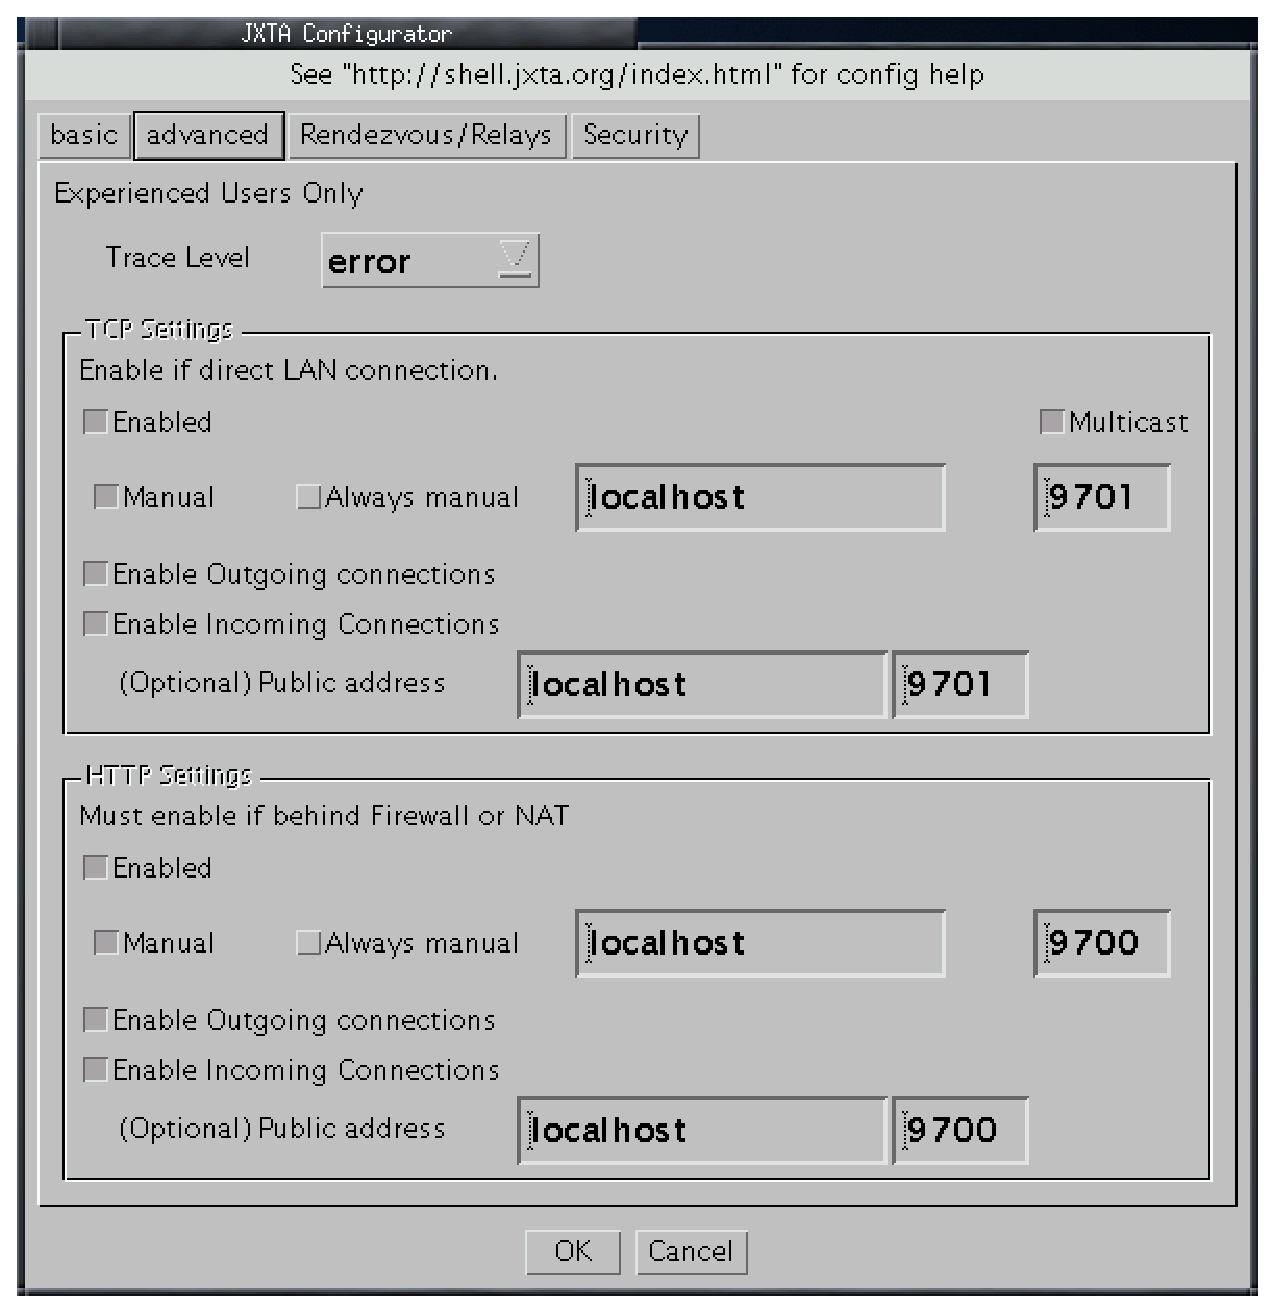
\includegraphics{fig/JXTAConfig}}
%%   \label{fig:platform}
  \caption{Configuring JXTA}
 \end{center}
\end{figure}

\item{\textbf{Second step}: registering a SeD to the MA. Be sure that
    the \texttt{parentName} inside the configuration file matches the
    name of the MA$_{DIET}$ previously launched. The command to run is:\\
    {\footnotesize \texttt{\$ java -cp <JXTA\_JARS> JXTASeD
        <DIET\_SeD\_config\_file> <computation\_abilities>}
    }\\
    If you want to put LA(s) between the MA and the
    SeD, launch the following command before loading the SeD:\\
    {\footnotesize
      \texttt{\$ java LA <DIET\_LA\_config\_file>}
    }\\ Check the DIET tree coherence and the \texttt{parentName}
    variables inside the configuration files. }
\item{\textbf{Third step}: Launch a client$_{J}$ with the command:\\
    {\footnotesize
      \texttt{\$ java -cp <JXTA\_JARS> JXTAClient <pb>}

   }
 }

  \end{itemize}
  

At this point, you still haven't tested the Multi-MA. To achieve this,
launch other MA$_{J}$(s) and launch again the client.

Scripts have been left at your disposal. You just need to check the
environment variables and paths required. As said before, only one
JXTA peer can be run in one directory, so each script is inside a
different one. These directories have to be edited (for
configuration), are named \texttt{MMA1/}, \texttt{MMA2/},
\texttt{MMA3/}, \texttt{LA1/}, \texttt{SeD1/}, \texttt{SeD2/} and
\texttt{client/}.  and are located in :
\texttt{<DIET\_root>/src/examples/JXTA/scripts}.



